\chapter{Our Proposal: An Operator based on Artificial Bees to Generate Diversity for Particle Swarm Optimization}\label{cap:contribution}
This chapter describes the operator proposed that was included in the APSO algorithm. This combination generated a algorithm proposed to be applied in problem very complex with search space of high dimensionality. The proposed algorithm, called \emph{Adaptive Bee and Particle Swarm Optimization} (ABeePSO), combines two classic well known swarm intelligence algorithms: APSO and ABC. The use of APSO is due to better convergence capability and some deficiencies were mitigated of the original PSO, with adaptive mechanisms based on the evolutionary factor. To maintain the diversity of swarm, we use the ABC algorithm because it performs the behavior change of employed bee to scout bee within the bee colony and allows the ability to escape from local minimum. Actually, the ABC algorithm was modified for this proposal. It used the calculation of centroid presents in the FSS algorithm to spread the bees in the search space.

\section{Motivation}
The APSO algorithm presents a more sophisticated mechanism to adapt the acceleration coefficients of the velocity equation based on the evolutionary factor, that was demonstrated an improvement in the convergence capability. However, the operator used to generate diversity (during the \emph{Jumping out} state) can be improved. The APSO Learning Strategy moves one particle per iteration and it does not provide enough diversity to solve more complicated problems (problems of high dimensionality).

However, some other swarm-based algorithms can deal more properly with this problem, such as the ABC that presents the capability to generate diversity when the guide bees are in the exploration mode. In this paper, we propose an approach to generate diversity by using the ABC when the APSO stagnates, i.e., to include the exploration ability of the ABC algorithm instead of using the Learning Strategy used in APSO. The swarm switches its behavior depending on a measurement of the diversity of the entire swarm.

\section{Adaptive Bee and Particle Swarm Optimization}
In our proposal, when the evolutionary state of the swarm is \emph{Convergence} the ABC algorithm is executed. Actually, it is an operator based on the ABC algorithm, that has the following steps: (i) guide bees movement; (ii) guided bees movement; and, (iii) classification of evolutionary state.

\subsection{Guide Bees Movement}
During the ABC execution, the first movement is performed by the guide bees, that it was inspired in the collective-volitive movement of FSS algorithm because used the centroid concept and expansion or contraction of the swarm in the search process (found in the subsection \ref{sse:FSS_volitive}). This movement guarantees the expansion of at least half of the swarm.

The swarm with $N$ particles is divided as follows. The $N/2$ particles with better fitness become guide bees and the other particles become guided bees. The $i^{th}$ guide bee will be optimized according to Equation (\ref{eq:ABeePSO_Guides}):

\begin{equation}\label{eq:ABeePSO_Guides}
{v}_{id} = {x}_{id} + step_d.{r}_{i}[{x}_{id} - B_d/d({x}_{id}, B_d)],
\end{equation}
 in which $B_d$ is the centroid of the guide bees, defined by Equation (\ref{eq:ABeePSO_Cent}), $step_d$ is the vector of dispersion steps of the swarm, determined by Equation (\ref{eq:ABeePSO_Step}), ${r}_{i}$ is a random number generated by an uniform distribution within the range [0,1] and $d(x_{id}, B_d)$ is the Euclidian distance between centroid ($B_d$) and current position ($x_{id}$).
\begin{equation}\label{eq:ABeePSO_Cent}
B_d = \frac{\sum^{N/2}_{i=1} x_{id}fit_{i}}{\sum^{N/2}_{i=1} fit_{i}},
\end{equation}
\begin{equation}\label{eq:ABeePSO_Step}
step_d = \{1-[1/(1+e^{\alpha(-f_{evol} + \beta)})]\}(x_d^{max} - x_d^{min}),
\end{equation}
where $x_d^{max}$ and $x_d^{min}$ are the lower and upper borders in the $d^{th}$ dimension of the search space, the displacement $\beta$ indicates the transition point of the logistic function and $\alpha$ is the sigmoid parameter.

Figure \ref{fig:ABeePSO_logistic} shows the graph of logistic function of dispersion step, with the values indicated. The reason of the use of logistic function is due to its characteristics. In more details, when the evolutionary factor value is small (that indicates the Convergence or Exploitation state of swarm) the step value $step_d$ is great, thus the swarm will expand faster. However, when the evolutionary factor is higher than 0.5, the step value is small. In this case, it is not necessary a high step value because the swarm is already spread. Thus, this avoids the explosion state of step value.

\begin{figure}[!h]
\centering
 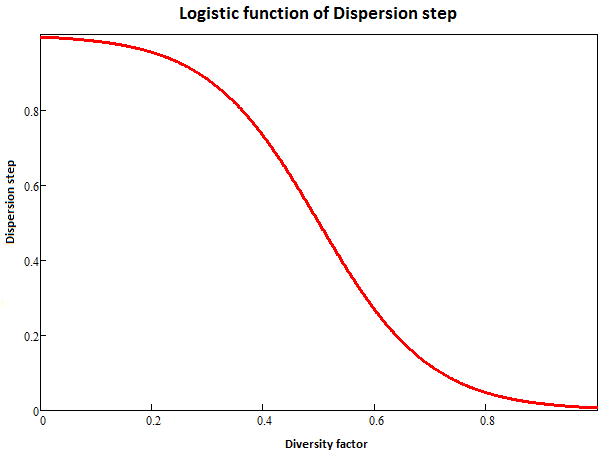
\includegraphics[width=0.65\textwidth]{image/Logistic.png}
 \caption{\small{Graphic illustration of logistic function of Dispersion step $step_d$.}}
 \label{fig:ABeePSO_logistic}
\end{figure}


When the fitness value changes, we update the value of the dispersion according to Equation (\ref{eq:ABeePSO_update}). If the new position is better than the current position, the step value is decreased because it found a good region; otherwise, the step value is increased.
\begin{equation} \label{eq:ABeePSO_update}
step_d = step_d \pm f_{evol}step_d.
\end{equation}

\subsection{Guided Bees Movement}
After the guide bee movement, the guided bees need to select one of the food sources, where the probability to choose a food source is given by Equation (\ref{eq:ABC_probability}). The guided bees movement is realized based on centroid ($B_d$) of swarm and the food source chosen to follow. Each guided bee searches for a new solution around the food source by using Equation (\ref{eq:ABeePSO_Guided}):
\begin{equation}\label{eq:ABeePSO_Guided}
v_{id} = x_{id} + r_{i}(fs_{id} - B_d),
\end{equation}
where $r_{i}$ is a random number within the range [0,1] and $fs_{id}$ is the food source selected by the guided bee.

\subsection{Classification of Evolutionary Factor}
The next step is to estimate the evolutionary state, such as in the APSO algorithm. However, this estimation just considers the food sources (half of swarm), which are the current potential solutions of the problem.

Figure \ref{fig:factor_ABeePSO} presents the membership functions used in our proposal. These fuzzy membership functions were defined through parameter analysis found in the Chapter \ref{cap:results}.
\begin{figure}[!h]
\centering
 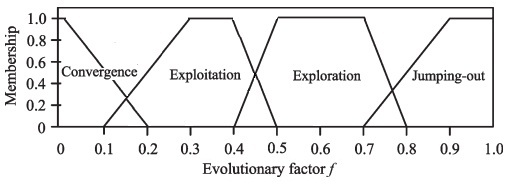
\includegraphics[width=0.65\textwidth]{image/factor_ABPSO}
 \caption{\small{Fuzzy membership functions for the ABeePSO algorithm.}}
 \label{fig:factor_ABeePSO}
\end{figure}

The classification of evolutionary state was altered in three of four evolutionary states: \emph{Convergence}, \emph{Exploitation} and \emph{Exploration}. Thus, the \emph{Jumping out} state has the same intervals of APSO algorithm. Then, we can observe the new values of intervals that have been changed to adapt the new diversity operator of our proposal.

\emph{Convergence State}: similar to the APSO algorithm, it occurs when the value of the evolutionary factor is very small and the particles are very close of the best particle. The algorithm is currently refining the solutions. However, the values of this state was altered because this operator spread at least half of the swarm. Thus, the occurrences of this state have to be decreased. We calculate the fuzzy value of this state according to Equation (\ref{eq:ABeePSO_convergence}).
\begin{equation}
S_{convergence}(f_{evol}) = \begin{cases}
1,                       & \mbox{if $0.0 \leq f_{evol} \leq 0.02$}, \\
(-f_{evol} + 0.2)/0.18,  & \mbox{if $0.02    < f_{evol} \leq 0.2$}, \\
0,                       & \mbox{if $0.2    < f_{evol} \leq 1.0$}.
\end{cases}
\label{eq:ABeePSO_convergence}
\end{equation}

\emph{Exploitation State}: as a APSO algorithm, it occurs when the value of the evolutionary factor is shrunk and the particles are near to the best particle. The values was modified to avoid the prolonged ABC execution and decrease convergence ability. The membership function of this state is defined according to Equation (\ref{eq:ABeePSO_exploitation}).
\begin{equation}
S_{exploitation}(f_{evol}) = \begin{cases}
0,                &\mbox{if $ 0.0 \leq f_{evol} \leq 0.1 $}, \\
5f_{evol} - 0.5,   &\mbox{if $ 0.1 <    f_{evol} \leq 0.3 $}, \\
1,                &\mbox{if $ 0.3 <    f_{evol} \leq 0.4 $}, \\
-10f_{evol} + 5,   &\mbox{if $ 0.4 <    f_{evol} \leq 0.5 $}, \\
0,                &\mbox{if $ 0.5 <    f_{evol} \leq 1.0 $}.
\end{cases}
\label{eq:ABeePSO_exploitation}
\end{equation}

\emph{Exploration State}: similar to the APSO algorithm, it occurs when the value of the evolutionary factor is ranging from medium to large and the particles have a medium or large distance of the best particle. The values of this state were altered with the same objective of the other states. We calculate the fuzzy value of this state according to Equation (\ref{eq:ABeePSO_exploration}).
\begin{equation}
S_{exploration}(f_{evol}) = \begin{cases}
0,                &\mbox{if $ 0.0 \leq f_{evol}  \leq 0.4 $}, \\
10f_{evol} - 4,    &\mbox{if $ 0.4   <  f_{evol}  \leq 0.5 $}, \\
1,                &\mbox{if $ 0.5   <  f_{evol}  \leq 0.7 $}, \\
-10f_{evol} + 8,  &\mbox{if $ 0.7   <  f_{evol}  \leq 0.8 $},  \\
0,                &\mbox{if $ 0.8   <  f_{evol}  \leq 1.0 $}.
\end{cases}
\label{eq:ABeePSO_exploration}
\end{equation}

The algorithm stops the execution of the ABC only when the evolutionary state is \emph{Jumping out} or \emph{Exploration}. During the execution of the ABC, the memory of the particles is stored. Before the restart of the APSO, it is necessary to compare the memory of the particles and the food sources. If the food source of the bee is better than the position stored in the memory, then the memory of the particle is updated, otherwise the memory is reestablished.

\subsection{Stagnation Counter}
This parameter works similarly the stagnation counter of ABC algorithm. It is a improvement of algorithm, because we observed that the ABeePSO algorithm lost the exploitation capability. The proposal uses like condition to execution of operator based on artificial bees the evolutionary state, \emph{i.e.},  when is \emph{Convergence} state, execute the modified ABC. Thus, the algorithm do not allow the deep exploration of the search region, because as from this moment the swarm expands.

Thus, the stagnation counter allows that swarm explore the search region during more iterations. Each particle has a stagnation counter. If the particle does not improve its position, this counter is increased. The combination of the stagnation counter with the evolutionary state guarantees a better exploitation ability.

\subsection{Pseudocode of the ABeePSO Algorithm}
The pseudocode of the ABeePSO algorithm is shown in Algorithm \ref{alg:ABeePSO}. In the pseudocode, we observe the same steps of APSO algorithm, but the lines 12 to 26 show the modified ABC. In the line 14 the guide bees movement is performed and the line 18 presents the guided bees movement.

\begin{algorithm}[!h]
    Initialize particles of swarm\;
    \While {the stop criterion is not achieved}{
        \For {each particle}{
            Evaluate the average distance according to Equation (\ref{eq:APSO_distance})\;
        }
        Calculate the evolutionary factor according to Equation (\ref{eq:APSO_factor})\;
        Calculate the membership function according to Equations (\ref{eq:ABeePSO_convergence}), (\ref{eq:ABeePSO_exploitation}), (\ref{eq:ABeePSO_exploration}) and (\ref{eq:s_jumpingout})\;
        Classify the swarm in the evolutionary state\;
        Adapt the acceleration coefficients according to Table \ref{tab:apso_strategies}\;
        Normalize the acceleration coefficients according to Equation (\ref{eq:APSO_normalized})\;
        Update the inertial factor according to Equation (\ref{eq:APSO_inertial})\;
        \If{classified on \emph{Convergence} state}
        {
           \While{Does not classified on \emph{Exploration} or \emph{Jumping out} state}
           {
                Execute guide bees movement according to Equation (\ref{eq:ABeePSO_Guides})\;
                \For {each guide bee}
                {
                    Calculate the probability od roulette wheel selection using the Equation (\ref{eq:ABC_probability})\;
                }
                Execute guided bees movement according to Equation (\ref{eq:ABeePSO_Guided})\;
                \For {each guide bee}{
                Calculate the average distance according to Equation (\ref{eq:APSO_distance})\;
                }
                Calculate the evolutionary factor according to Equation (\ref{eq:APSO_factor})\;
                Calculate the membership function according to Equations (\ref{eq:ABeePSO_convergence}), (\ref{eq:ABeePSO_exploitation}), (\ref{eq:ABeePSO_exploration}) and (\ref{eq:s_jumpingout})\;
                Classify the swarm in the evolutionary state\;
           }
        }
        Update the memory of particles using food sources\;
        \For {each particle}
        {
            Update the social memory in neighborhood\;
            Update the velocity according to Equation (\ref{eq:PSO_velocity})\;
            Update the position according to Equation (\ref{eq:PSO_position})\;
            Evaluate the position using the objective function of problem\;
            \If{current position is better than cognitive memory}
            {
                Update the cognitive memory\;
            }
            \If{current position is better than social memory}
            {
                Update the social memory\;
            }
        }
    }
    \Return the social memory.
    \caption{Pseudocode of the ABeePSO algorithm.}
    \label{alg:ABeePSO}
\end{algorithm}

\section{Clan Adaptive Bee and Particle Swarm Optimization}
The Clan Adaptive Bee and Particle Swarm Optimization (ClanABeePSO) is an algorithm that presents the characteristics of our proposed algorithm with communication topology of clans, found in the ClanPSO algorithm. Similar to the ClanAPSO algorithm, the use of the cooperative behavior with multi swarm system allows that the sub-swarms can perform different types of search by iteration of the algorithm. It is possible to observe different types of agents (particles and bees) as well.

As the ClanPSO algorithm, each clan use a fully-connected structure. However, for each iteration, each one of clans performs a search using the ABeePSO algorithm and selects the particle with the best information of the entire clan (delegation of leader). The leaders adjust their positions running a APSO or PSO execution and the conference can be performed using either global or local topology.

\subsection{Pseudocode of the ClanABeePSO Algorithm}
The simplified pseudocode of the ClanABeePSO algorithm is shown in Algorithm \ref{alg:ClanABeePSO}. In lines 3 to 6 have the ABeePSO execution within each clan. But, the other parts of pseudocode are similar to the ones presented in the ClanAPSO algorithm.

\begin{algorithm}[!h]
    Initialize the particles with random positions and velocities\;
    \While {the stop criterion is not achieved}{
        \For {each clan}{
            Execute ABeePSO within the clans\;
            Delegate leader\;
        }
        Create conference of leaders\;
        Execute APSO (or PSO) with the leaders\;
    }
    \Return the best particle.
    \caption{Pseudocode of ClanABeePSO algorithm.}
    \label{alg:ClanABeePSO}
\end{algorithm}
\pagebreak
